\def\multisequencebound{MS\xspace}
\def\msbound{\multisequencebound}


\newcommand{\cut}[1]{}

In previous versions of \osprey, the \ks algorithm~\cite{K*} modeled an ensemble of Boltzmann-weighted conformations to approximate the Boltzmann-weighted partition function. It combined minimized dead-end elimination pruning~\cite{DEE} with \as~\cite{DEE,A*} gap-free conformation enumeration to compute provable $\varepsilon$-approximations to the partition function for the protein and ligand states of interest. \ks combined these partition function scores to approximate the association constant, \ka, as the ratio of $\varepsilon$-approximate partition functions between the bound and unbound states of a protein-ligand complex. Notably, each partition function ratio, called a \ks \emph{score}, is provably accurate with respect to the biophysical \emph{input model}~\cite{K*,minDEE,iMinDEE}. 

Although \ks efficiently and provably approximates \ka for a given sequence, it must compute a \ks score for each sequence of interest. All provable ensemble-based algorithms, as well as many heuristic algorithms which optimize binding affinity, are \emph{single-sequence} algorithms which must compute the binding affinity for each possible sequence. Therefore, designs with many mutable residues rapidly become intractable. \osprey 3.0 provides a new algorithm, \bbks, which overcomes this challenge. \bbks~\cite{BBK*} builds on \ks, and is the first provable, ensemble-based protein design algorithm to run in time sublinear in the number of sequences. The key innovation in \bbks that enables this improvement is the \emph{multi-sequence (\msbound) bound}. Rather than compute binding affinity separately for each possible sequence, as single-sequence methods do, \bbks efficiently computes a single provable \ks score upper bound for a combinatorial number of sequences. \bbks uses \msbound bounds to prune a combinatorial number of sequences during the search, entirely avoiding single-sequence computation for all pruned sequences.

Importantly, \bbks also contains many other powerful algorithmic improvements and implementation optimizations: the parallel architecture of \bbks, which enables concurrent energy minimization, and a novel two-pass partition function bound, which minimizes far fewer conformations while still computing a provable $\varepsilon$-approximation to the partition function. Combined with the combinatorial pruning power of the \msbound bound, \bbks is able to search over sequence spaces two orders of magnitude larger than previously possible with single-sequence \ks, and is up to 1700 times more efficient~\cite{BBK*} (Fig.~\ref{fig:bbks}). Not only is \bbks able to provably bound and prune a combinatorial number of suboptimal sequences, \bbks also provably approximates \ks scores for individual sequences up to three orders of magnitude faster than single-sequence \ks~\cite{BBK*}. These improvements show that \bbks not only accelerates protein designs that are possible with previous provable algorithms, it also efficiently performs designs that are too large for previous methods.

\begin{figure}
\center
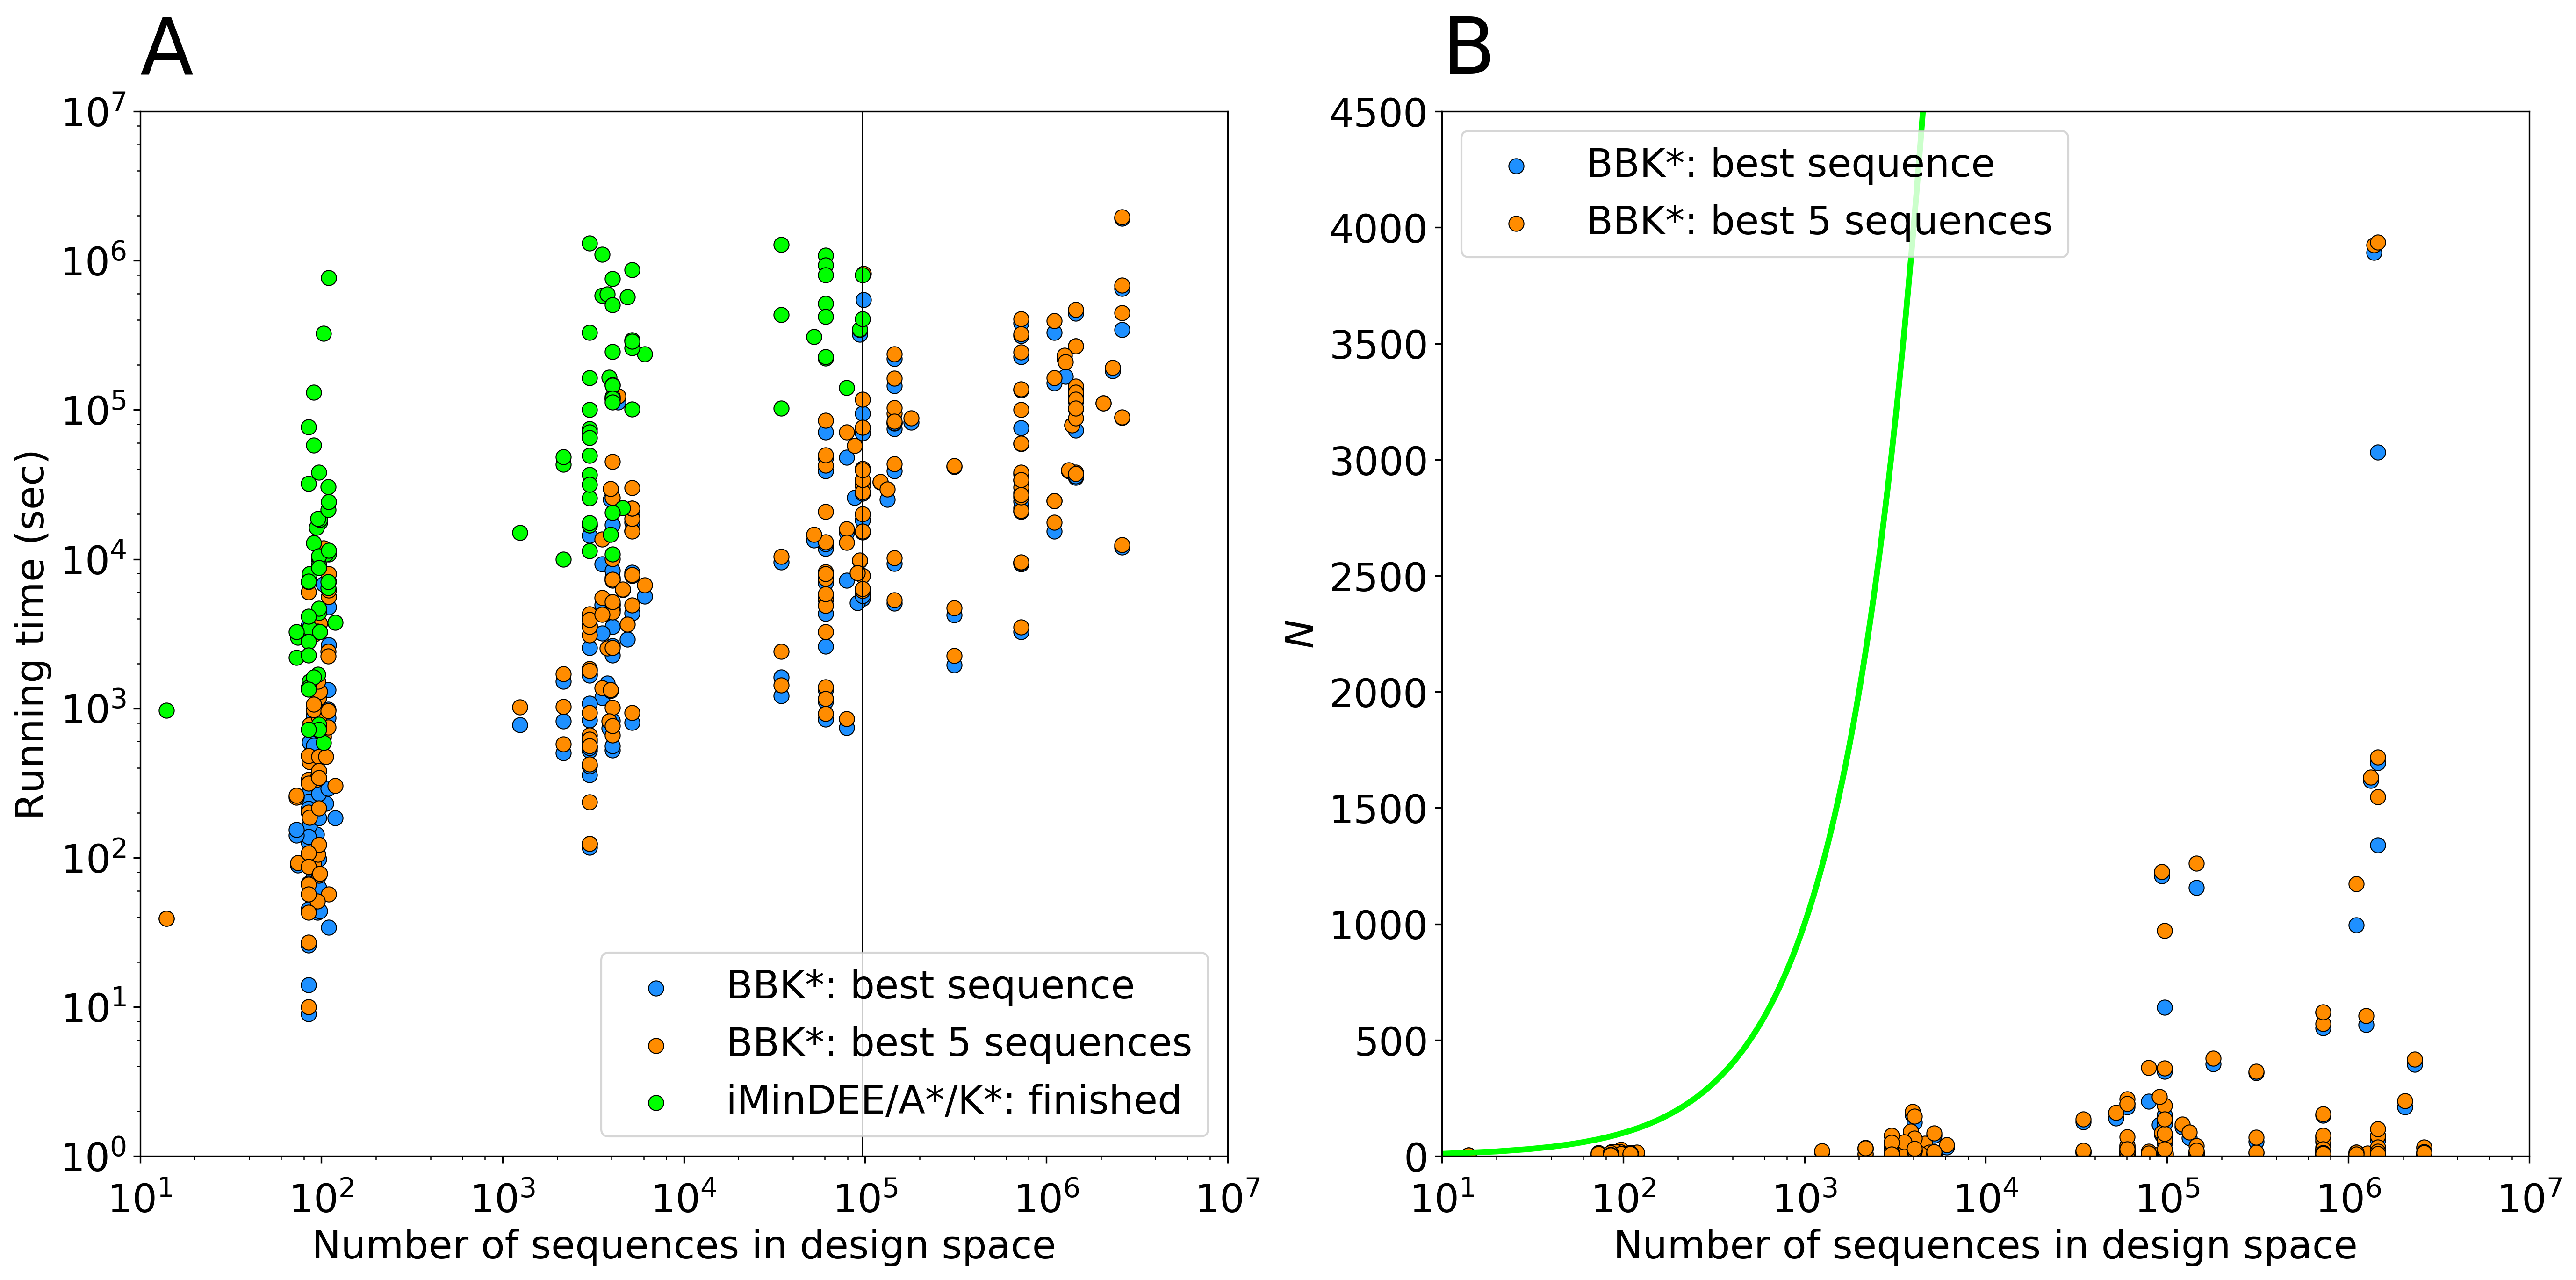
\includegraphics[width=4in]{figures/bbks.png}
\caption{Running times for \bbks and single-sequence \ks vs. the number of sequences in the search space for 204 protein design test cases, described in Ref.~\citen{BBK*}.  Single-sequence \ks completed only 107 of the test cases within the 30-day time limit (left of the vertical line), and took up to 800 times longer than \bbks to do so, while \bbks completed all the designs within the time limit.  Figure reprinted with permission from Ref.~\citen{BBK*}.  }
\label{fig:bbks}
\end{figure}
